\section{Method}\label{sec:method}
% Spatial correlation 2d histograms (den nemme, 1 2d hist)
In this section, we will describe the method for exploiting spatial correlation based of the 2D-histograms of the tomographies.
We will start by motivating the problem, then give an overview of how we solve the problem, with the final detailed walkthrough of each step of the overall workflow.

\subsection{1-dimensional histograms}
%diskuter overlappende materialer
If we look at a 1D-histogram of a tomography, as shown in~\Cref{fig:1d-hist}, we see that it is hard to globally threshold which material belongs to which voxel intensity.
This is because the voxel intensity is not a globally defined value, as explained in~\Cref{sec:physics}, which means that the different materials cover ranges of intensities, which blend together in the histogram.
Instead, we should exploit the spatial information in the tomography, as the intensities varies according based of off their positioning.

\begin{figure}
    \centering
    \carl{TODO 1D histogram of a tomography. Skal måske have nogle fordelinger "fittet" ind, så man kan se overlappet?}
    \caption{1-dimensional histogram of a tomography. The x-axis depicts voxel intensity.}
    \label{fig:1d-hist}
\end{figure}

\subsection{Correlation of the different angles}
%Show the correlation of x,y,z,r to histograms 2d
In order to include spatial information, we consider \textit{expanding} a dimension to produce multiple 1D histograms.
Each histogram is computed by locking the dimension in question and produce the 1D histogram, combining these for each entry in the expanded axis into a new 2-dimensional histogram.
We consider expanding four different axes of the tomography: x, y, z and radius (r).
Each of them can be computed with a single pass over the entire tomography, as the code in~\Cref{alg:2dhists} shows.
%\carl{Which is better?~\Cref{lis:2dhists} or~\Cref{alg:2dhists}. I know the algorithm has more information, but it could easily be added to the listing as well.}

%discuss the effects with references to the physics (previous section)
\carl{ref til section 2.4}

% Kept for historical reasons.
%\begin{figure}
%    \begin{lstlisting}[language=Python,caption=Python-like pseudo code for computing 2D histograms.,label=lis:2dhists]
%for z, y, x in indices:
%    v = voxels[z,y,x]
%    r = int(sqrt((x-cx)**2 + (y-cy)**2))
%    zhist[z,v] += 1
%    yhist[y,v] += 1
%    xhist[x,v] += 1
%    rhist[r,v] += 1
%    \end{lstlisting}
%\end{figure}

\begin{algorithm}
    \caption{2-dimensional histograms. Allocation also implies zero initialization.}
    \label{alg:2dhists}
    \begin{algorithmic}
        \Function {2D\_hist} {$voxels[n_z,n_y,n_x],c_x,c_y,n_{bins},v_{min},v_{max}$}
            \State $n_r \gets \left\lfloor\sqrt{\left\lfloor \frac{n_x}{2} \right\rfloor^2 + \left\lfloor \frac{n_y}{2} \right\rfloor^2}\right\rfloor+1$
            \State \textbf{allocate} $h_z[n_z,n_{bins}], h_y[n_y,n_{bins}]$
            \State \textbf{allocate} $h_x[n_x,n_{bins}], h_r[n_r,n_{bins}]$
            \For {$z,y,x$ \textbf{in} $0{:}n_z,0{:}n_y,0{:}n_x$}
                \State $v \gets voxels[z,y,x]$
                \If {$v_{min} \leq v \leq v_{max}$}
                    \State $v_{i} \gets (n_{bins}-1) \cdot \frac{v - v_{min}}{v_{max} - v_{min}}$
                    \State $r \gets \left\lfloor\sqrt{(x-c_x)^2 + (y-c_y)^2}\right\rfloor$
                    \State $h_z[z,v_{i}]{+}{+}$
                    \State $h_y[y,v_{i}]{+}{+}$
                    \State $h_x[x,v_{i}]{+}{+}$
                    \State $h_r[r,v_{i}]{+}{+}$
                \EndIf
            \EndFor
            \Return $h_z,h_y,h_z,h_r$
        \EndFunction
    \end{algorithmic}
\end{algorithm}

The four expanded histograms can be seen in~\Cref{fig:2dhists}.
We can see that the different expansions divide the materials differently, based on where in the tomography we look.
E.g. the top part of the \texttt{y} histogram only has a single distinquishable material, whereas the bottom part carries multiple clearly distinquished materials.

\begin{figure}
    \centering
    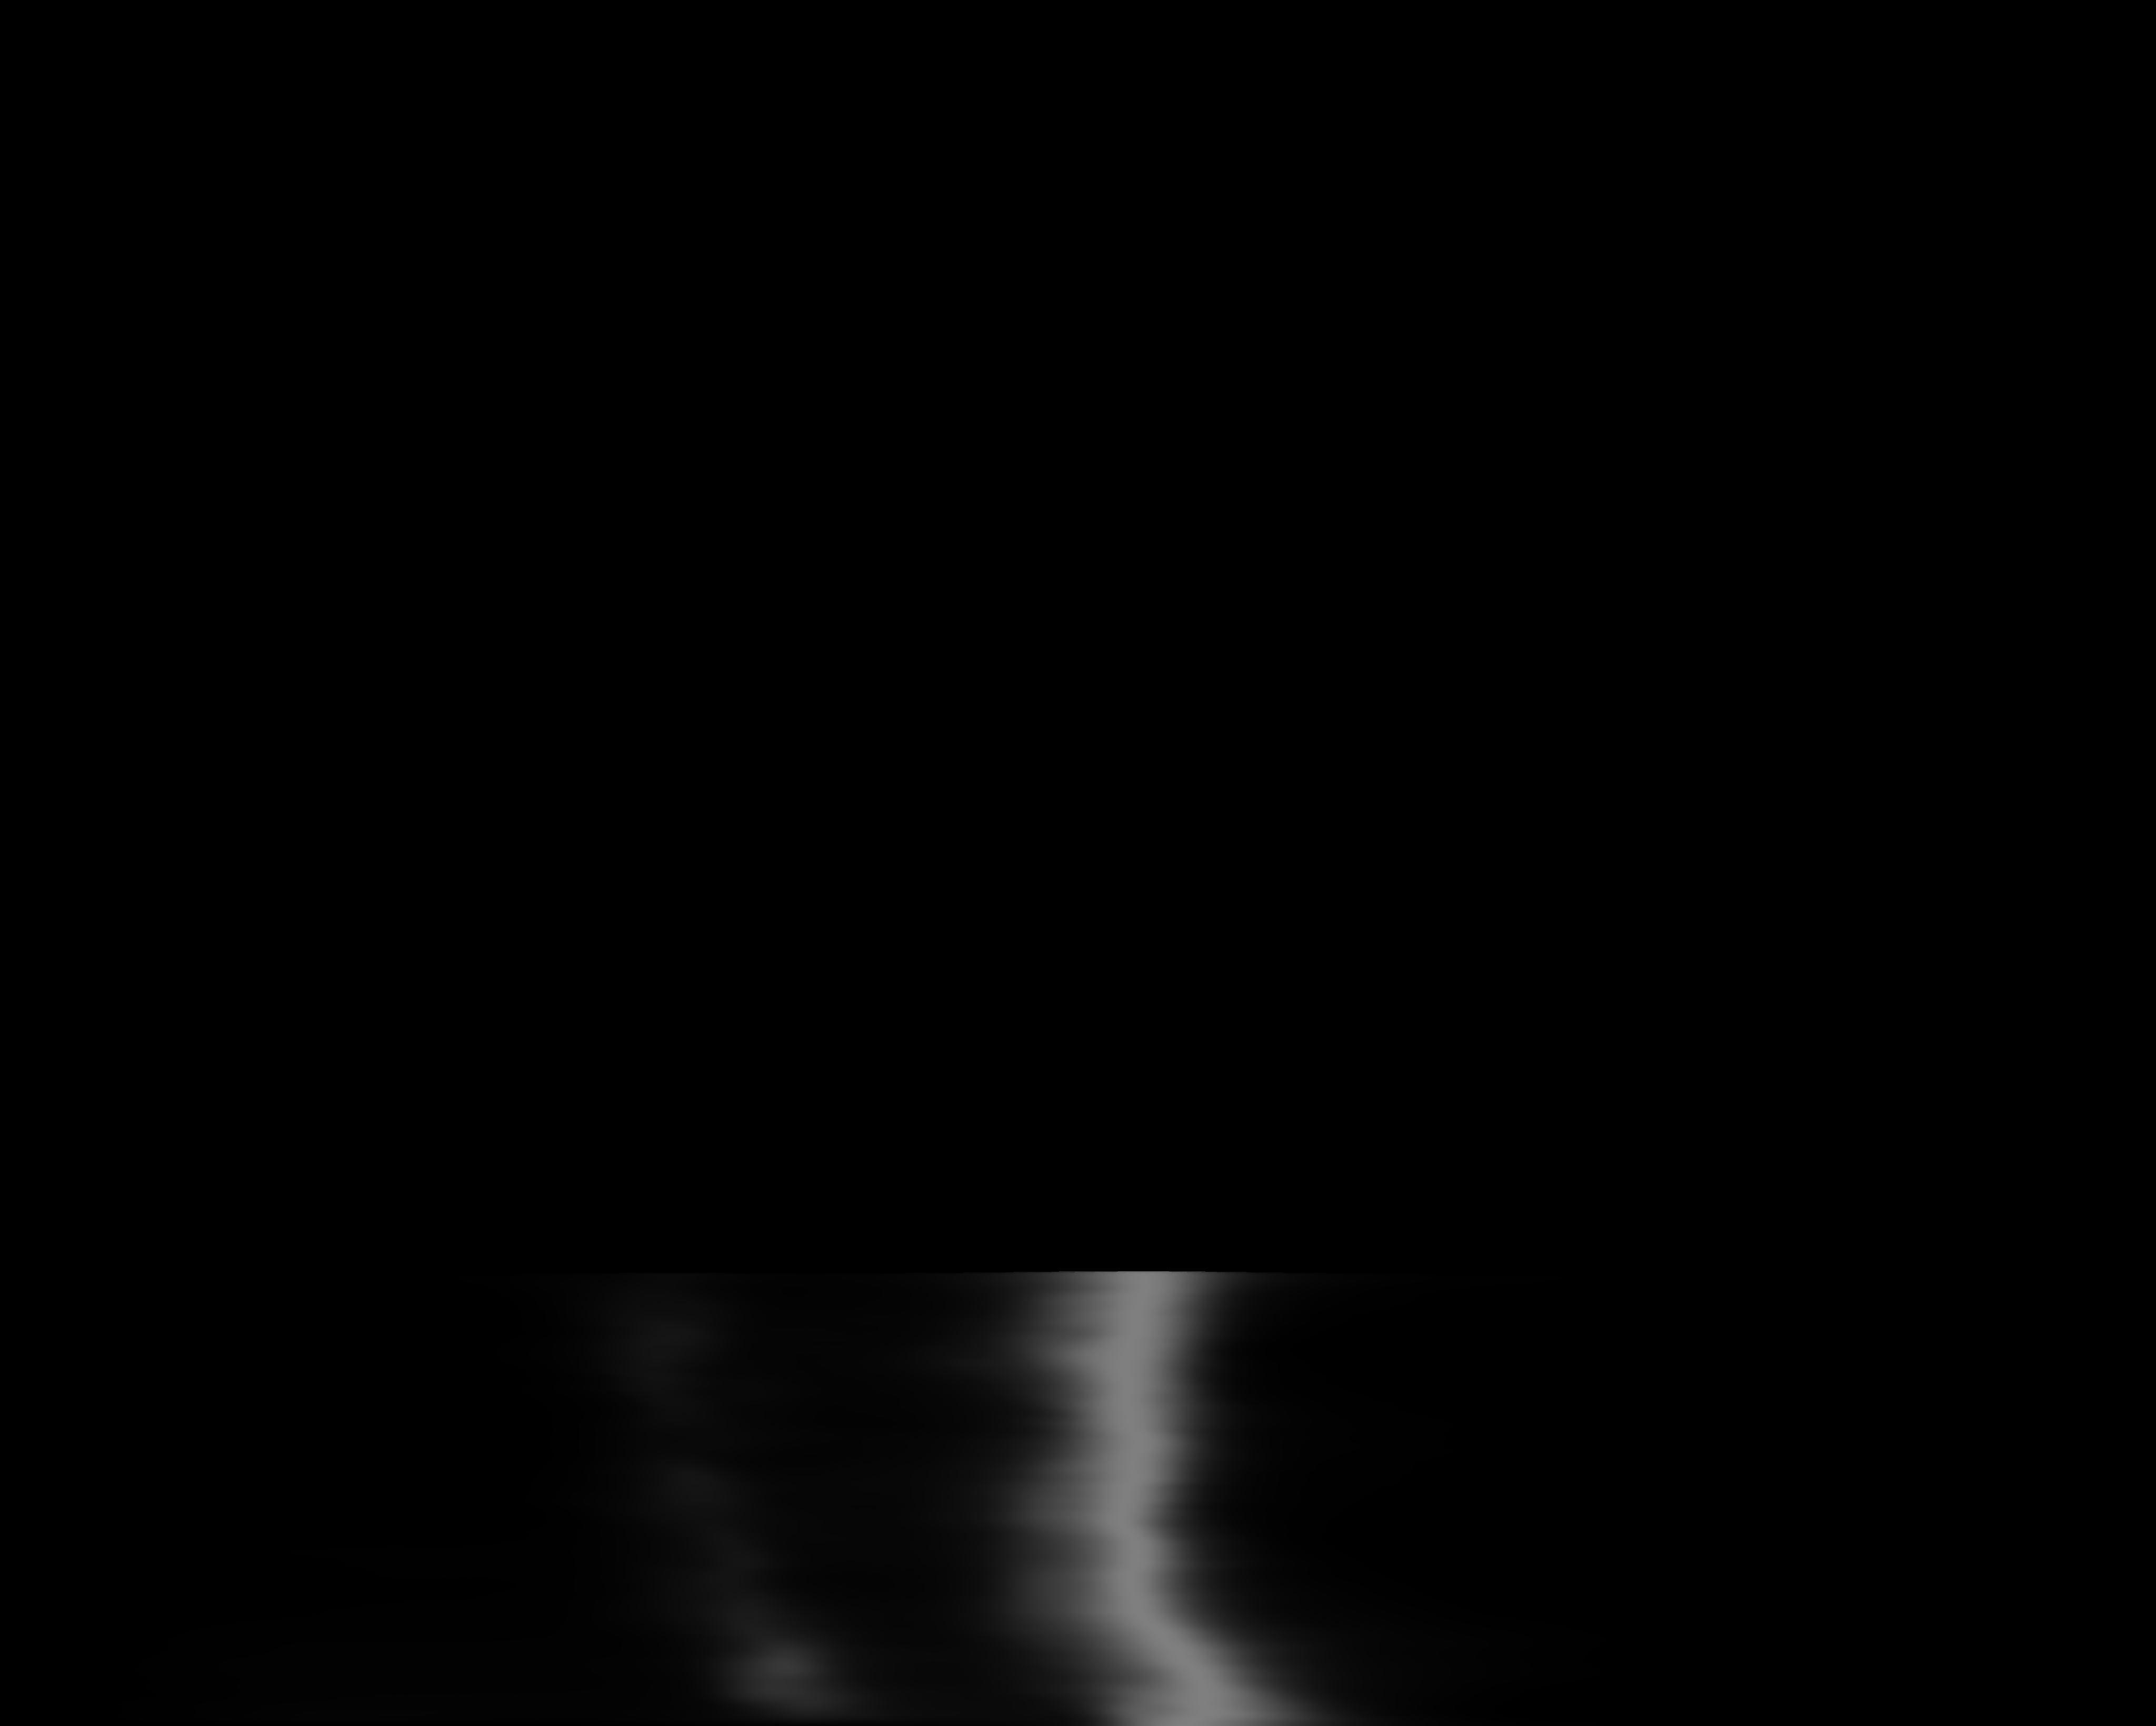
\includegraphics[width=.49\linewidth]{figures/zb-bone_region3.png}
    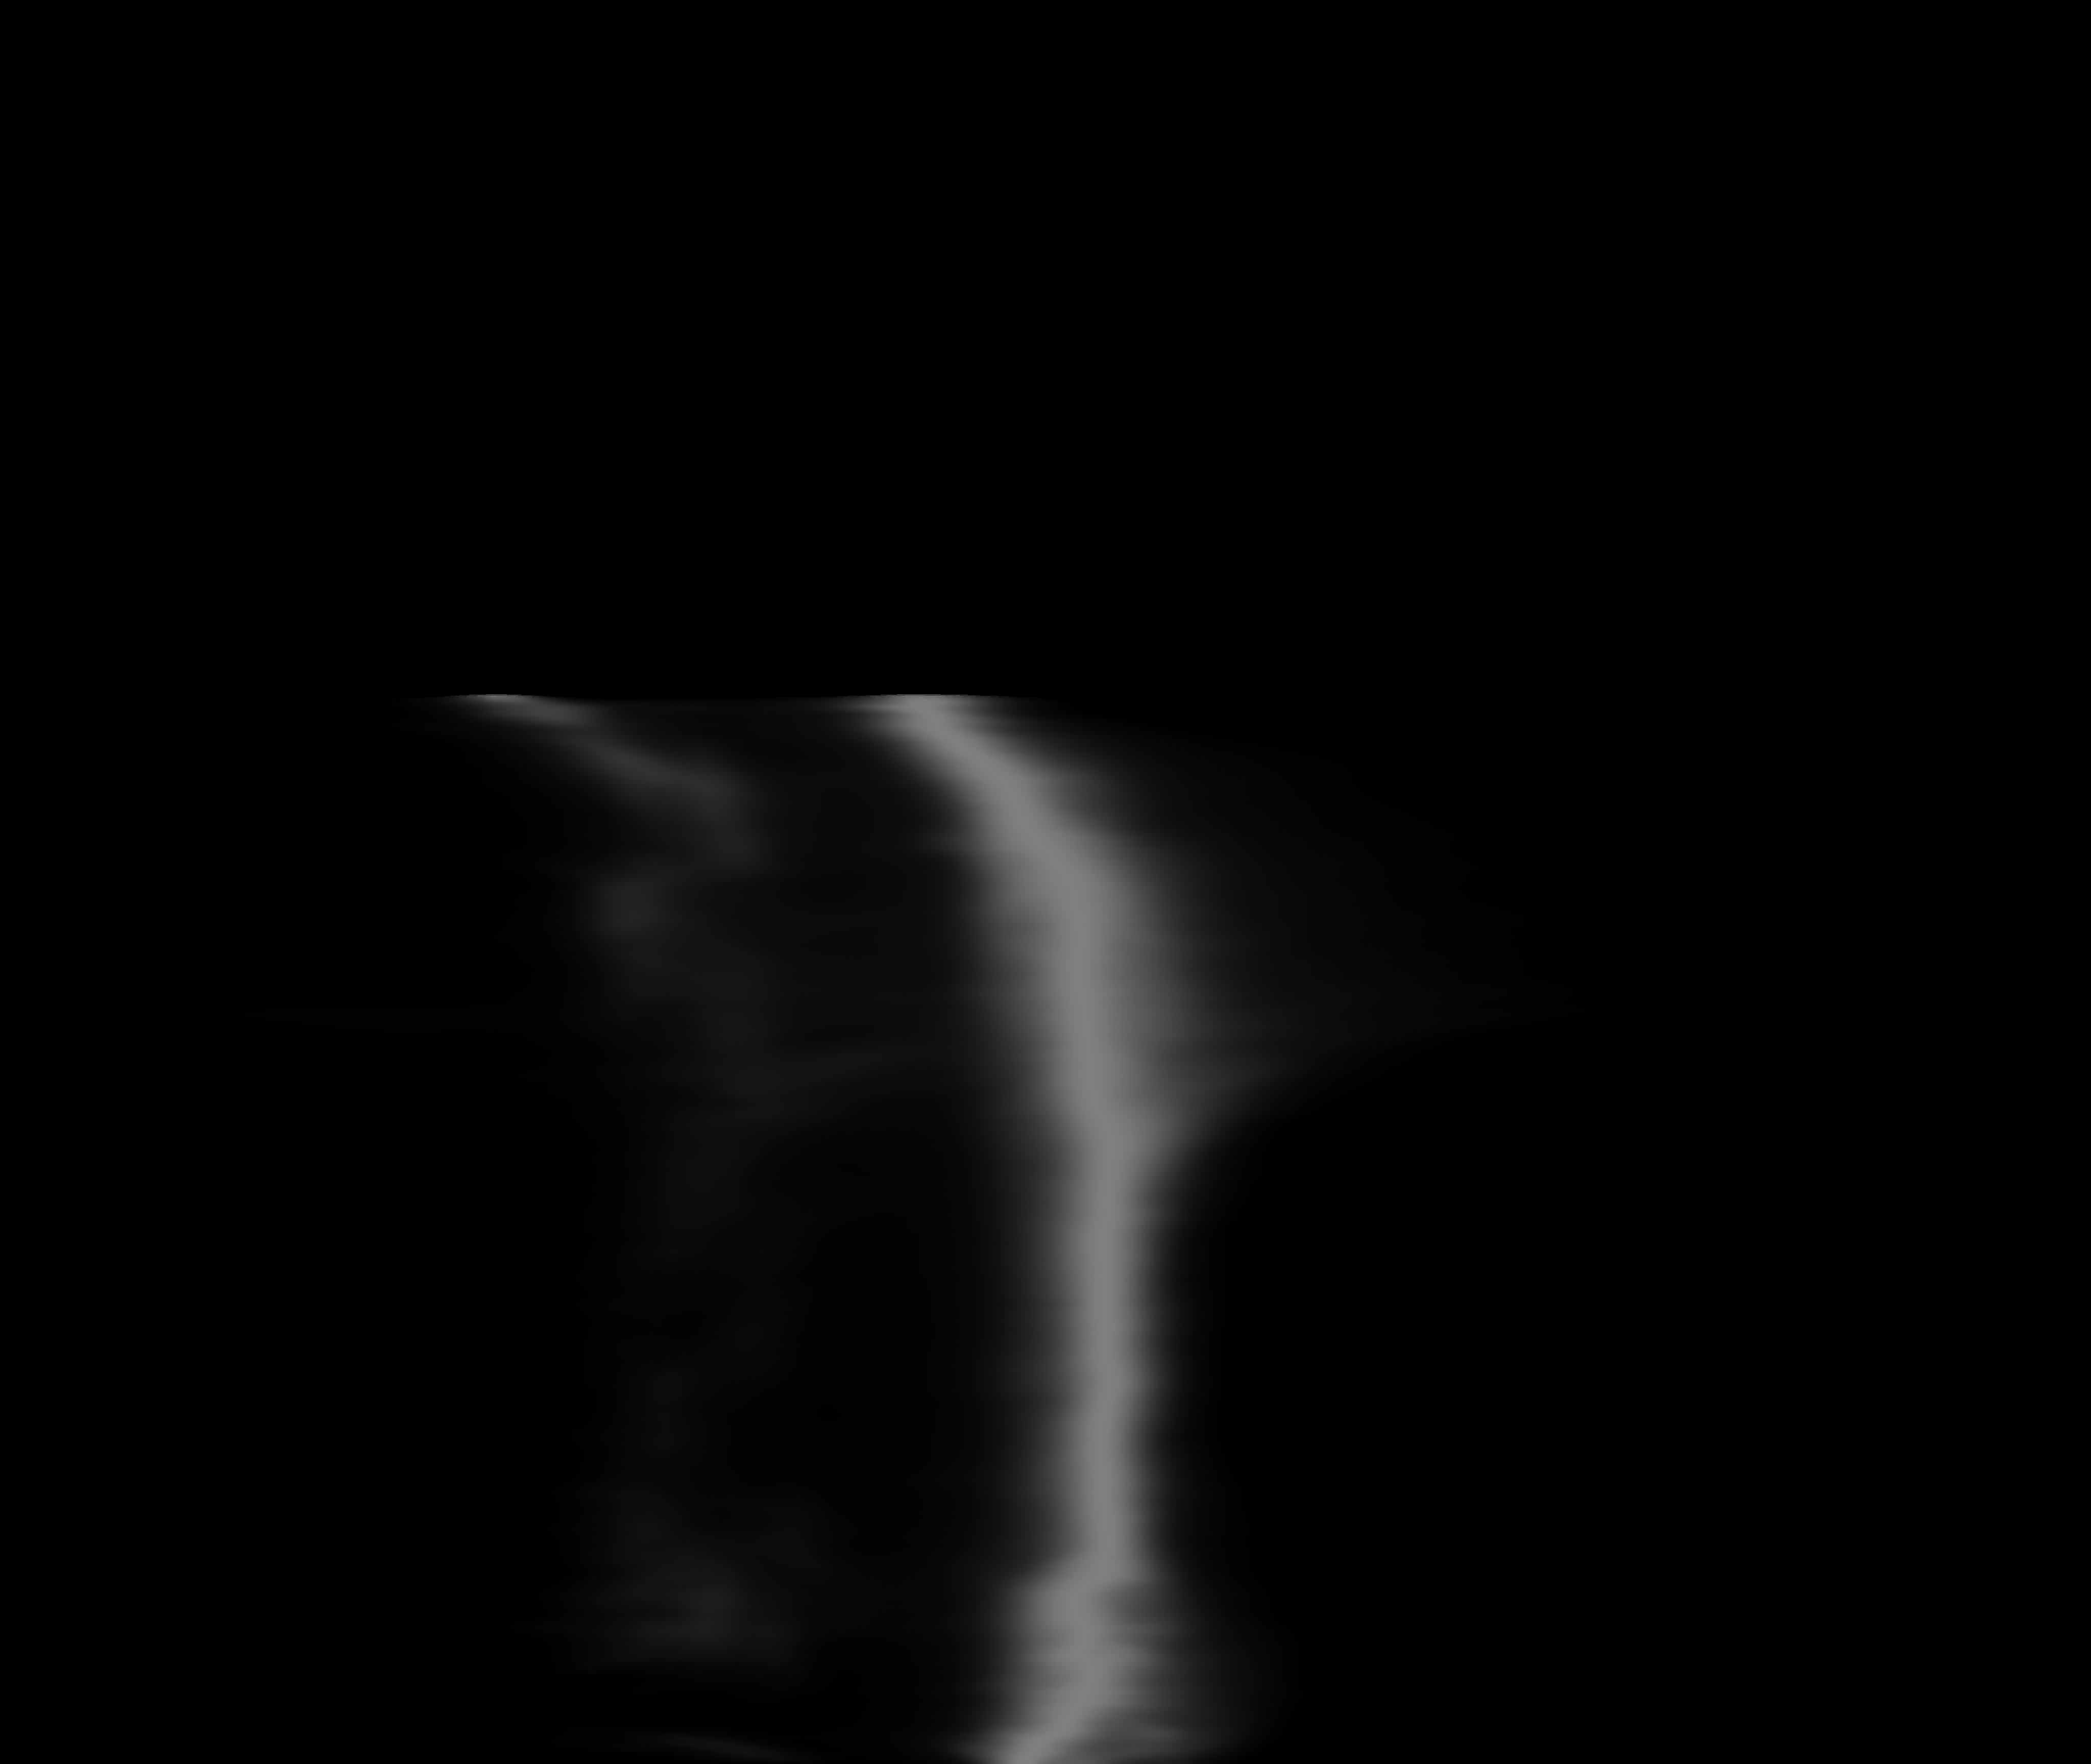
\includegraphics[width=.49\linewidth]{figures/yb-bone_region3.png}
    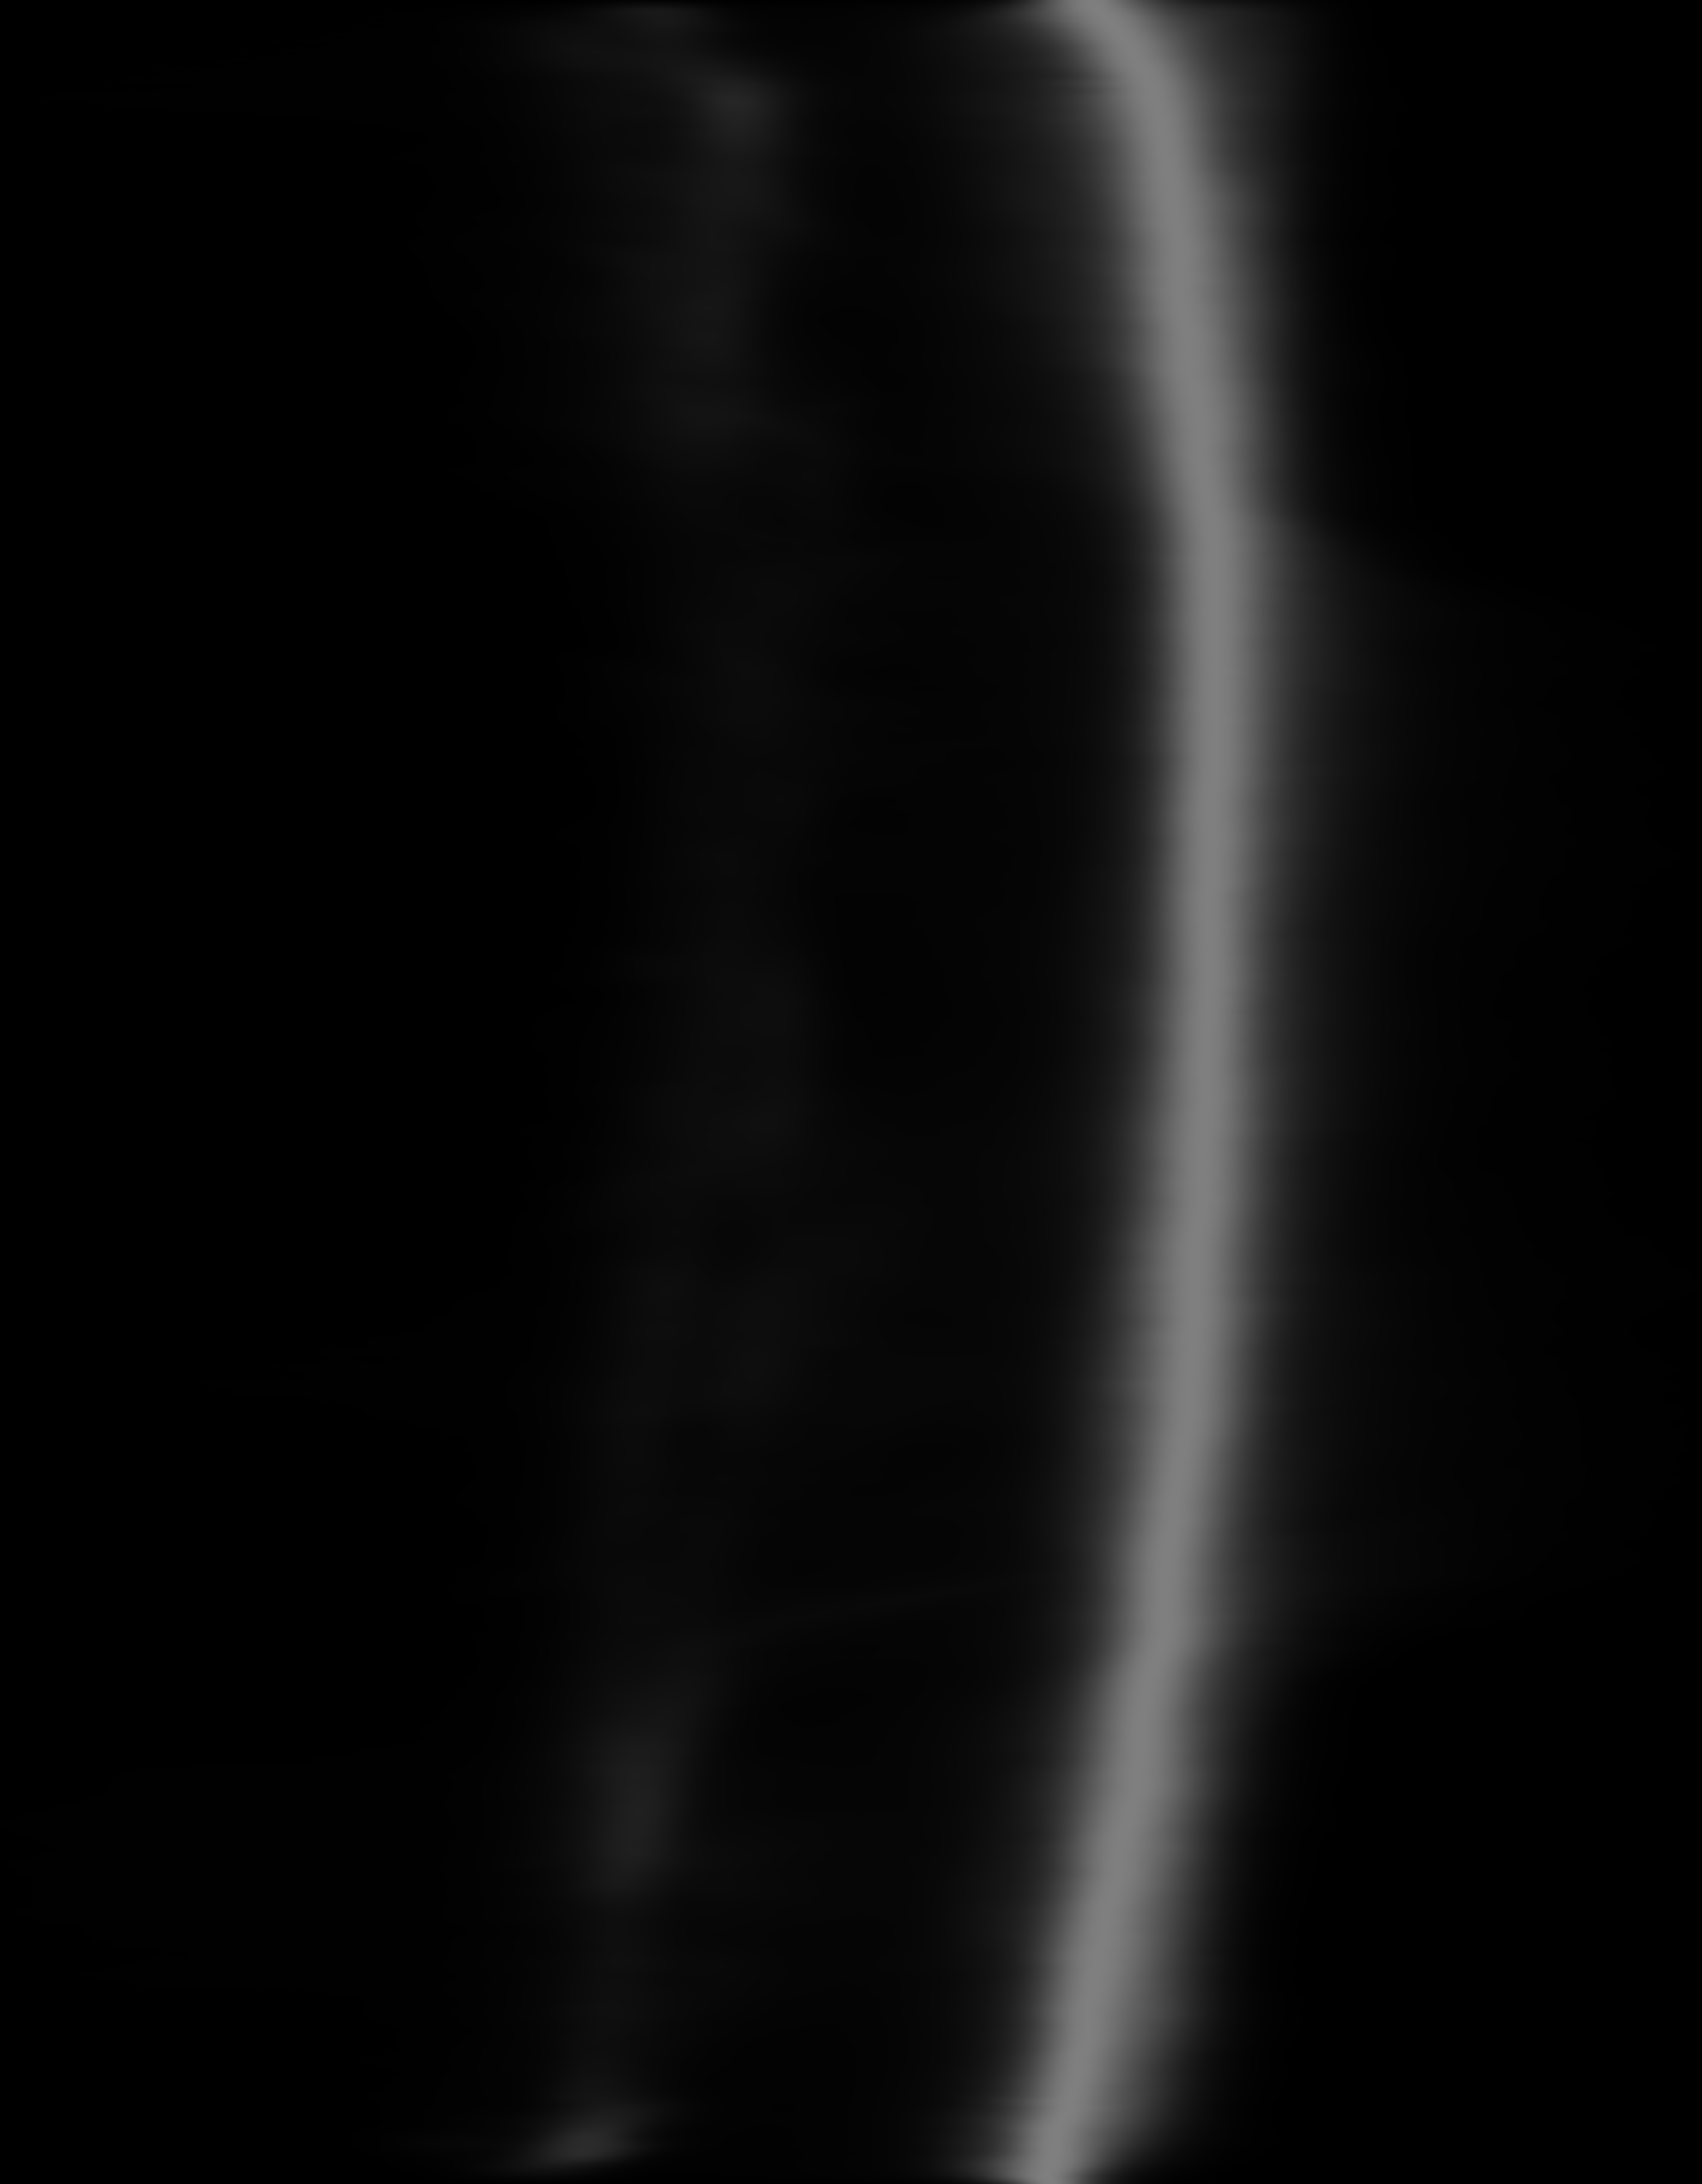
\includegraphics[width=.49\linewidth]{figures/xb-bone_region3.png}
    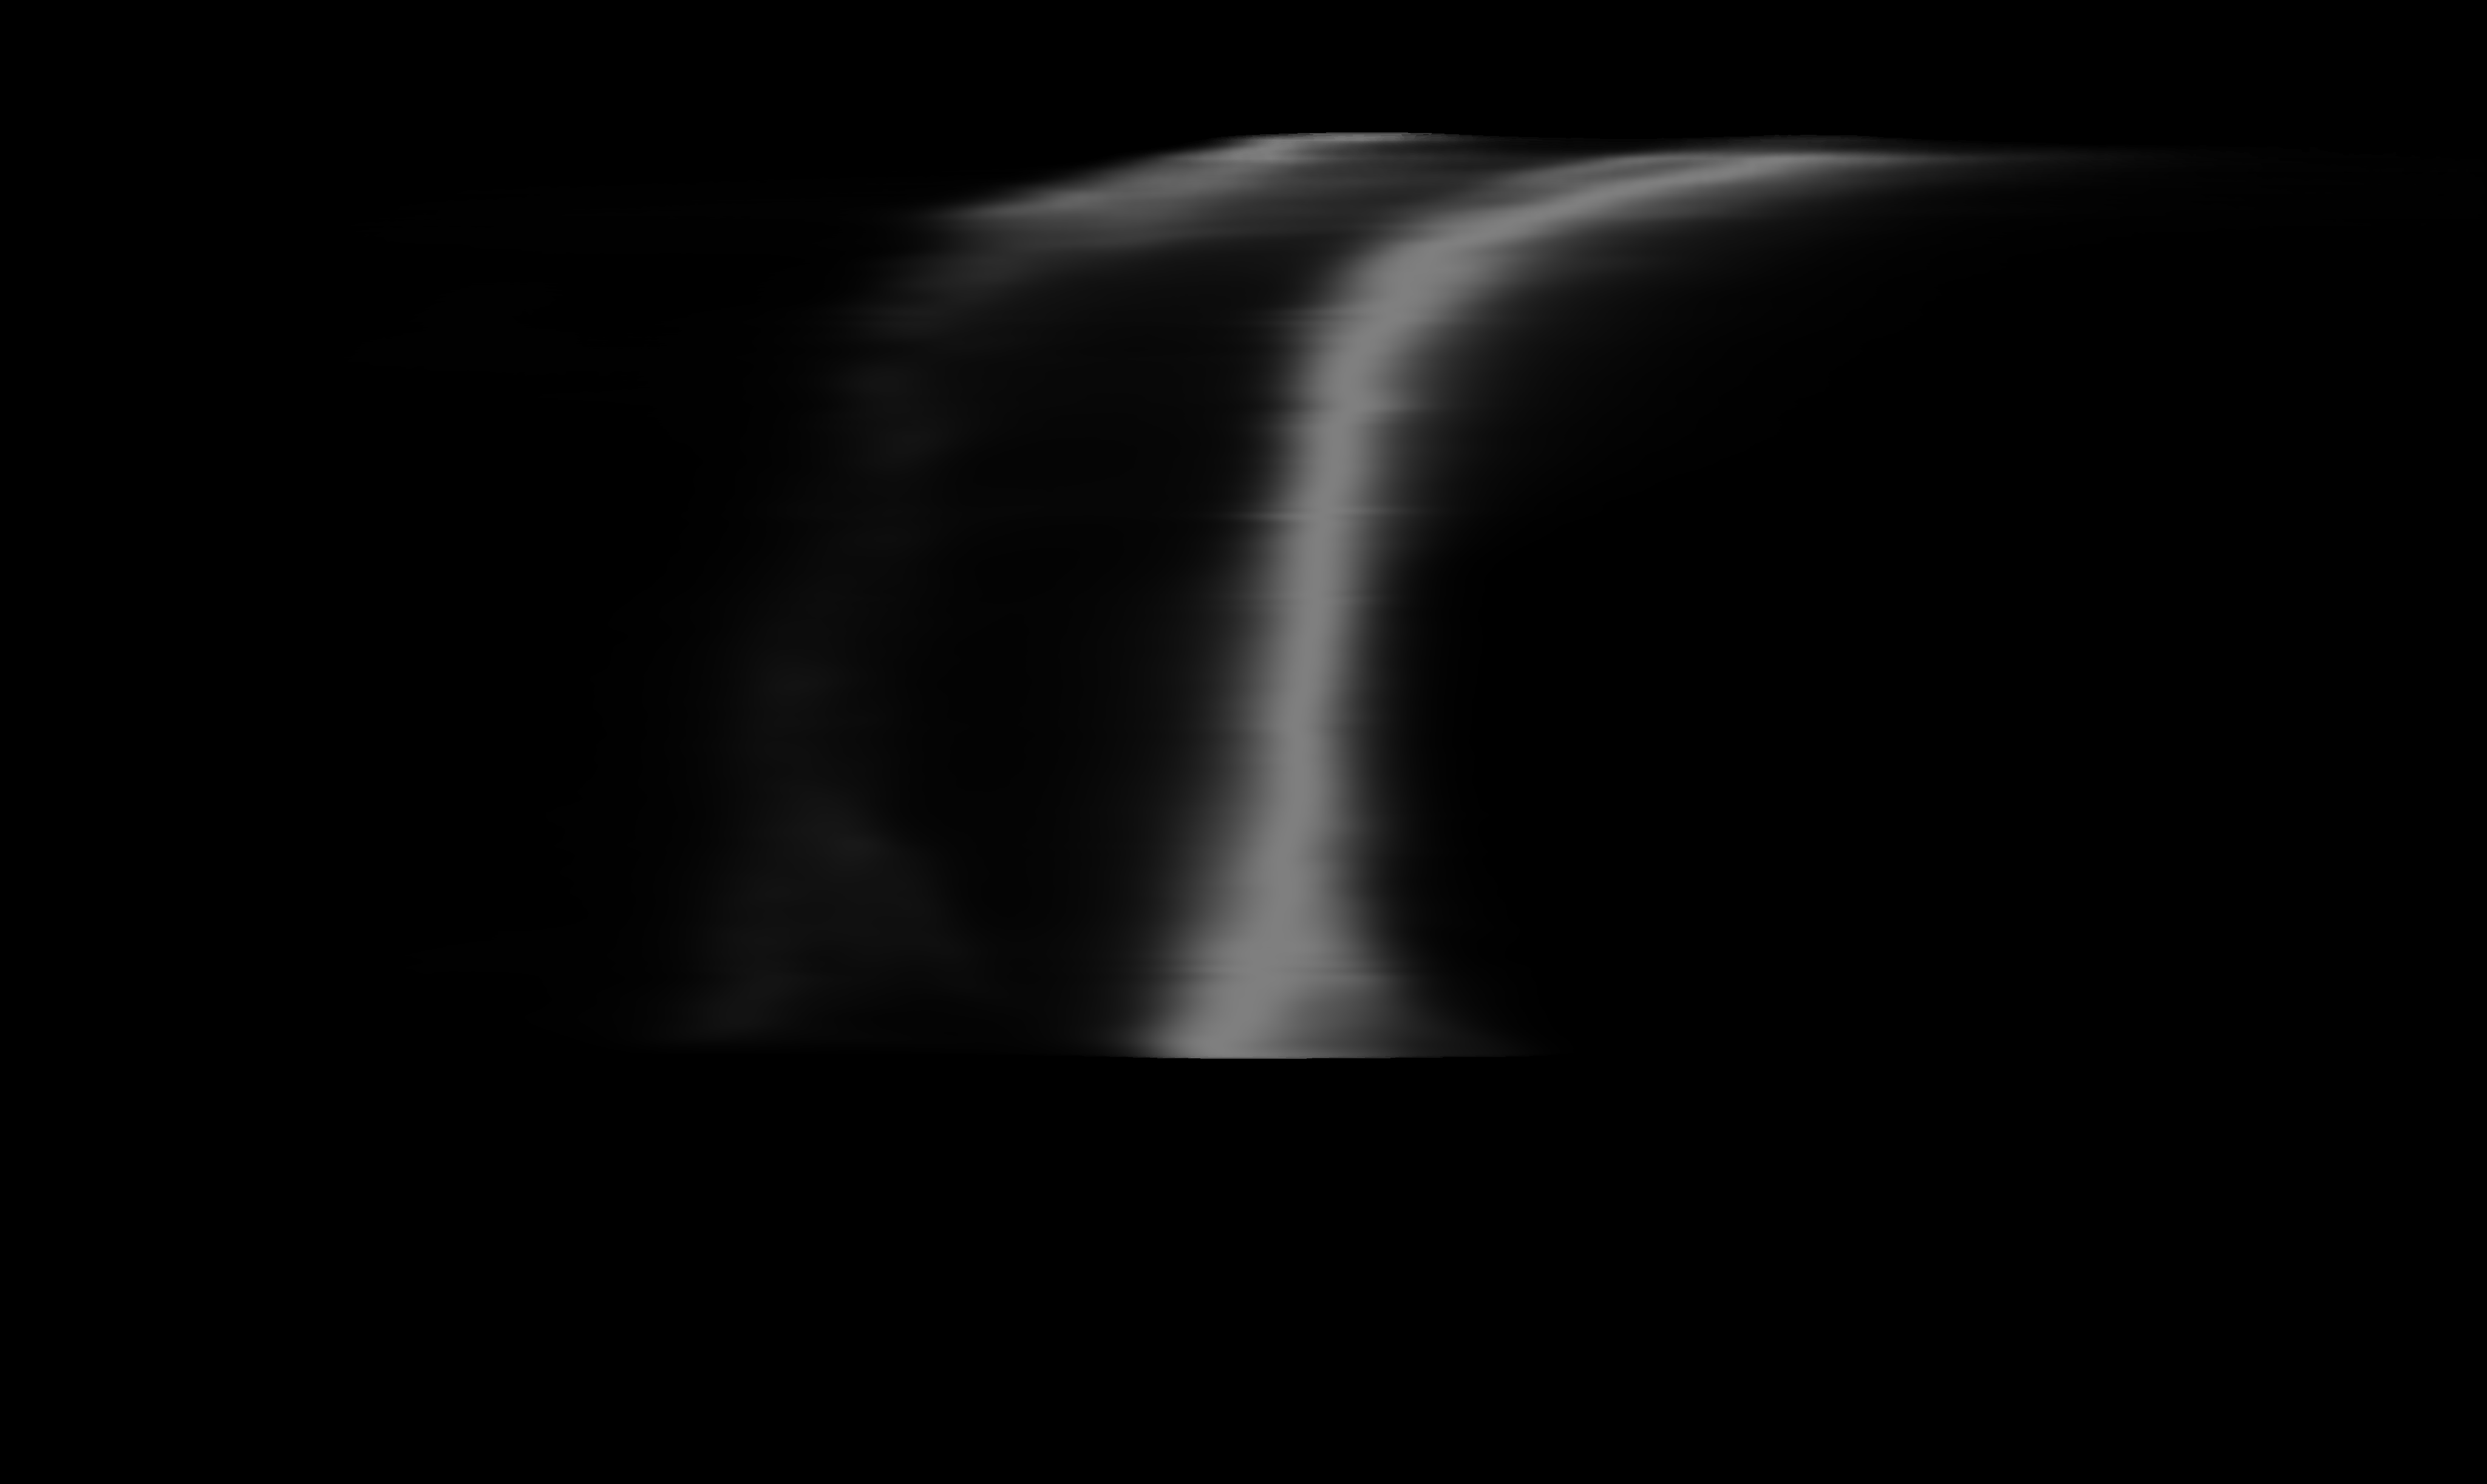
\includegraphics[width=.49\linewidth]{figures/rb-bone_region3.png}
    \caption{2D histograms of the different dimension expansions. Top row: z and y. Bottom row: x and r. \carl{Change the color scheme, add axes ticks.}}
    \label{fig:2dhists}
\end{figure}

\subsection{Removing unnecessary information.}
\carl{Mention how we apply the implant and bone masks? Or should it be before, so that the x,y,z,r histograms are also 2 materials?}

\subsection{EDT, diffusion}
%Show that the fields can perfectly seperate
%discuss all the way to implant contact
While the four histograms further seperate the materials at different angles, they are not good at depicting the materials close to the implant.
\carl{I'm not really sure that's the reason for field histogramming? Isn't it more like for this simple case, it does a well enough job, as the bayesian approach would be the optimal?}

In order to obtain spatial information based on the relation to the implant, we construct two \emph{field} representations: Euclidian Distance Transform (EDT) and Diffusion.

%EDT is good overall, but difficult close to the implant.
EDT computes each voxel as the euclidian distance to the implant. This makes for a generally good representation for all but the voxels that are close to the implant. This is mainly due to the fact that the voxels in the grooves of the implant gets the same value as the voxels next to the threads of the implant, as is shown in~\Cref{fig:edt-vs-diffusion}.

%Use diffusion to "zoom in" on the implant, as it is good close to the implant, but throws everything far away into the same bin
To zoom in on the implant, we utilize diffusion where the implant "glows" further accumulating the value when a voxel is surrounded by implant. This is shown in~\Cref{fig:edt-vs-diffusion}, where the voxels in the grooves are affected by multiple implant voxels.

\begin{figure}
    \centering
    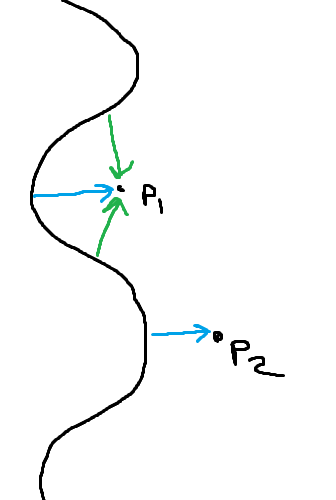
\includegraphics[width=.7\linewidth]{figures/edt-diffusion.png}
    \caption{High-quality render of the different field computations close to the implant in the YZ plane. The EDT is depicted in blue, where we see that $p_1$ and $p_2$ has the same distance. Diffusion is depicted in green, where we see multiple arrows contributing to the value of $p_1$. \carl{TODO: actual render.}}
    \label{fig:edt-vs-diffusion}
\end{figure}

While Diffusion works well on voxels close to the implant, it assigns the same value to the voxels far from the implant. As such, an optimal solution is to use both the EDT and the diffusion field to better represent both voxels that are far away, as well as the ones that are close to the implant.

%Show that the distance to the implant in edt will be the same in the grooves of the screw compared to the threads of the screw. This is "fixed" with diffusion, as the grooves will be brigher as it is surrounded by more implant.

\subsection{Walkthrough of the method}
This section will describe the steps of the method for going from tomography to material probability distributions.
%\carl{flavortext}

\subsubsection{Overview}
%Coarse steps, explain the idea
The steps of the segmentation method are:
\begin{enumerate}
    \item Compute the EDT and Diffusion fields to give each voxel spatial information about its relation to the implant.
    \item Compute frequency distributions of voxel values as functions of field values
      as 2D histograms.
    \item Find the materials within the 2D histograms as ridges, using image processing techniques.
    \item From the ridges, compute initial approximate frequence distributions of each material,
      which are then optimized to fit the 2D histograms. From the optimized distributions, we derive
      probability distributions for material classification.
\end{enumerate}
The computed distributions approximate the conditional probabilities $P(m|v,x)$ that a particular voxel
is material $m$ given that it has value $v$ and field value $x$. 

\james{TODO: Forklar bedre. Adskil ny segmenteringsmetode og anvendelse til BIC}

These steps are also summarized in the flow chart in~\Cref{fig:flowchart}.

\begin{figure}
    \centering
    \begin{tikzpicture}
        \node[draw] (field) at (0,0) {Compute fields};
        \node[draw, below = of field] (hists) {Compute 2D histograms};
        \node[draw, below = of hists] (curvs) {Find Curves};
        \node[draw, below = of curvs] (probs) {Compute probabilities};
        \node[draw, below = of probs] (segm)  {Segment the voxels};
        \node[draw, below = of segm]  (blood) {Compute blood network};
        \node[draw, below = of blood] (bic)   {Compute bone- and blood-implant contact};

        \path[draw, ->] (field) -- (hists);
        \path[draw, ->] (hists) -- (curvs);
        \path[draw, ->] (curvs) -- (probs);
        \path[draw, ->] (probs) -- (segm);
        \path[draw, ->] (segm) -- (blood);        
        \path[draw, ->] (blood) -- (bic);
    \end{tikzpicture}
    \caption{Flowchart depicting the steps of the method.
%    \carl{Skal nok labeles, så man nemt kan se hvilken section der beskriver det. Plus, teksten i kasserne nok også kan være mere flavorful!}
    \carl{Kan måske arrangeres ligesom Davids ting oversigt? Giver måske kun mening hvis der var mere end bare segmentation -> bic}}
    \label{fig:flowchart}
\end{figure}

\subsubsection{Segmentation}
Now we will list each step detailing the actual implementation for segmentation. The steps for segmentation are steps 1-5.
%\carl{better flavortext}

\vspace{\baselineskip}
\noindent\textit{\textbf{1. Field computations}}
\carl{mention implant mask}

EDT

For diffusion, rather than solving the diffusion equation, we approximate using multiple convolutions of a 3D-gaussian kernel.
Instead of a single pass with a 3D-kernel, we apply 3 1D convolutions, one in each dimension, to the tomography, obtaining the same result as a regular 3D kernel.
The pseudo code can be seen in~\Cref{alg:diffusion}, with x, y, and z slices in~\Cref{fig:field-slices}

%\begin{figure}
%    \begin{lstlisting}[language=Python,caption=Python-like pseudo code for the diffusion approximation.,label=lis:diffusion]
%S = [Ny*Nx, Nx, 1]
%N = [Nz, Ny, Nx]
%for rep in repitions:
%    for dim in dimensions:
%        for z, y, x in indices:
%            X = [z,y,x]
%            is = -min(k, X[dim])
%            ie = min(k, N[dim]-X[dim]-1)
%            idx = z*S[0] + y*S[1] + x*S[2]
%            for i in range(is,ie):
%                in_idx = idx + i*S[dim]
%                output[idx] +=
%                    voxels[in_idx] * kernel[i+k]
%    \end{lstlisting}
%\end{figure}

\begin{algorithm}
    \caption{Diffusion approximation.}
    \label{alg:diffusion}
    \begin{algorithmic}
        \Function {Diffusion} {$voxels[n_z*n_y*n_x], repitions, kernel[2*k+1]$}
            \State $S \gets [n_y * n_x, n_x, 1]$
            \State $N \gets [n_z, n_y, n_x]$
            \State \textbf{allocate} $buf_0[n_z*n_y*n_z], buf_1[n_z*n_y*n_x]$
            \State $buf_0[:] \gets voxels[:]$
            \For {$rep$ \textbf{in} $repitions$}
                \For {$dim$ \textbf{in} $dimensions$}
                    \For {$z,y,x$ \textbf{in} $0{:}n_z,0{:}n_y,0{:}n_x$}
                        \State $X \gets [z,y,x]$
                        \State $i_{start} \gets - \min (k, X[dim])$
                        \State $i_{end} \gets \min (k, N[dim] - X[dim] - 1)$
                        \State $i_{global} \gets z*S[0] + y*S[1] + x*S[2]$
                        \For {$i$ \textbf{in} $i_{start}:i_{end}$}
                            \State $i_{offset} \gets i_{global} + i*S[dim]$
                            \State $buf_1[index] \gets buf_0[i_{offset}] * kernel[i+k]$
                        \EndFor
                    \EndFor
                    \State $buf_0[:] \gets buf_1[:]$
                \EndFor
            \EndFor
            \Return $buf_0$
        \EndFunction
    \end{algorithmic}
\end{algorithm}

\begin{figure}
    \carl{TODO show x, y, and z slices of the EDT and Diffusion field. Either each field seperate or combined?}
    \caption{Slices of the EDT field at different collapsed dimensions.}
    \label{fig:field-slices}
\end{figure}

%EDT + Diffusion
To obtain good seperation both close to the implant and far away, we combine the two fields into a single one.
\carl{TODO how is this actually done? Or should it just be that both are used during segmentation, each contributing 50 \%? As in, let the probabilities for each of them "take over"}

\carl{(remember to show images)}

\vspace{\baselineskip}
\noindent\textbf{2D histograms} \\

From these fields, we compute 2D histograms with the voxel value on the x-axis and field value on the y-axis.
This allows us to see the distribution of voxel values, based off their relative position from the implant.
The pseudo code can be seen in~\Cref{alg:field-hist} with a plot of the resulting histogram in~\Cref{fig:field-hist}.
We see that the voxel intensities shift based off how close to the implant they are, which indicates that a global threshold would not be sufficient.

%\begin{figure}
%    \begin{lstlisting}[language=Python,caption=Python-like pseudo code for computing the 2D field histograms.,label=lis:field-hist]
%for z, y, x in indices:
%    v = voxel[z,y,x]
%    f = field[z,y,x]
%    hist[f,v] += 1
%    \end{lstlisting}
%\end{figure}

\begin{algorithm}
    \caption{Field 2D histograms.}
    \label{alg:field-hist}
    \begin{algorithmic}
        \Function {Field\_hist} {$voxels[n_z,n_y,n_x], field[n_z,n_y,n_x],$ \newline $v_{bins}, v_{min}, v_{max}, f_{bins}, f_{min}, f_{max}$}
            \State \textbf{allocate} $h[v_{bins},f_{bins}]$
            \For {$z,y,x$ \textbf{in} $0{:}n_z,0{:}n_y,0{:}n_x$}
                \State $v \gets voxels[z,y,x]$
                \If {$v_{min} \leq v \leq v_{max}$}
                    \State $f \gets voxels[z,y,x]$
                    \If {$f_{min} \leq f \leq f_{max}$}
                        \State $v_i \gets (v_{bins} - 1) - \frac{v - v_{min}}{v_{max} - v_{min}}$
                        \State $f_i \gets (f_{bins} - 1) - \frac{f - f_{min}}{f_{max} - f_{min}}$
                        \State $h[f_i,v_i]{+}{+}$
                    \EndIf
                \EndIf
            \EndFor
            \Return $h$
        \EndFunction
    \end{algorithmic}
\end{algorithm}
\carl{look at indenting the function arguments in~\Cref{alg:field-hist}}

\begin{figure}
    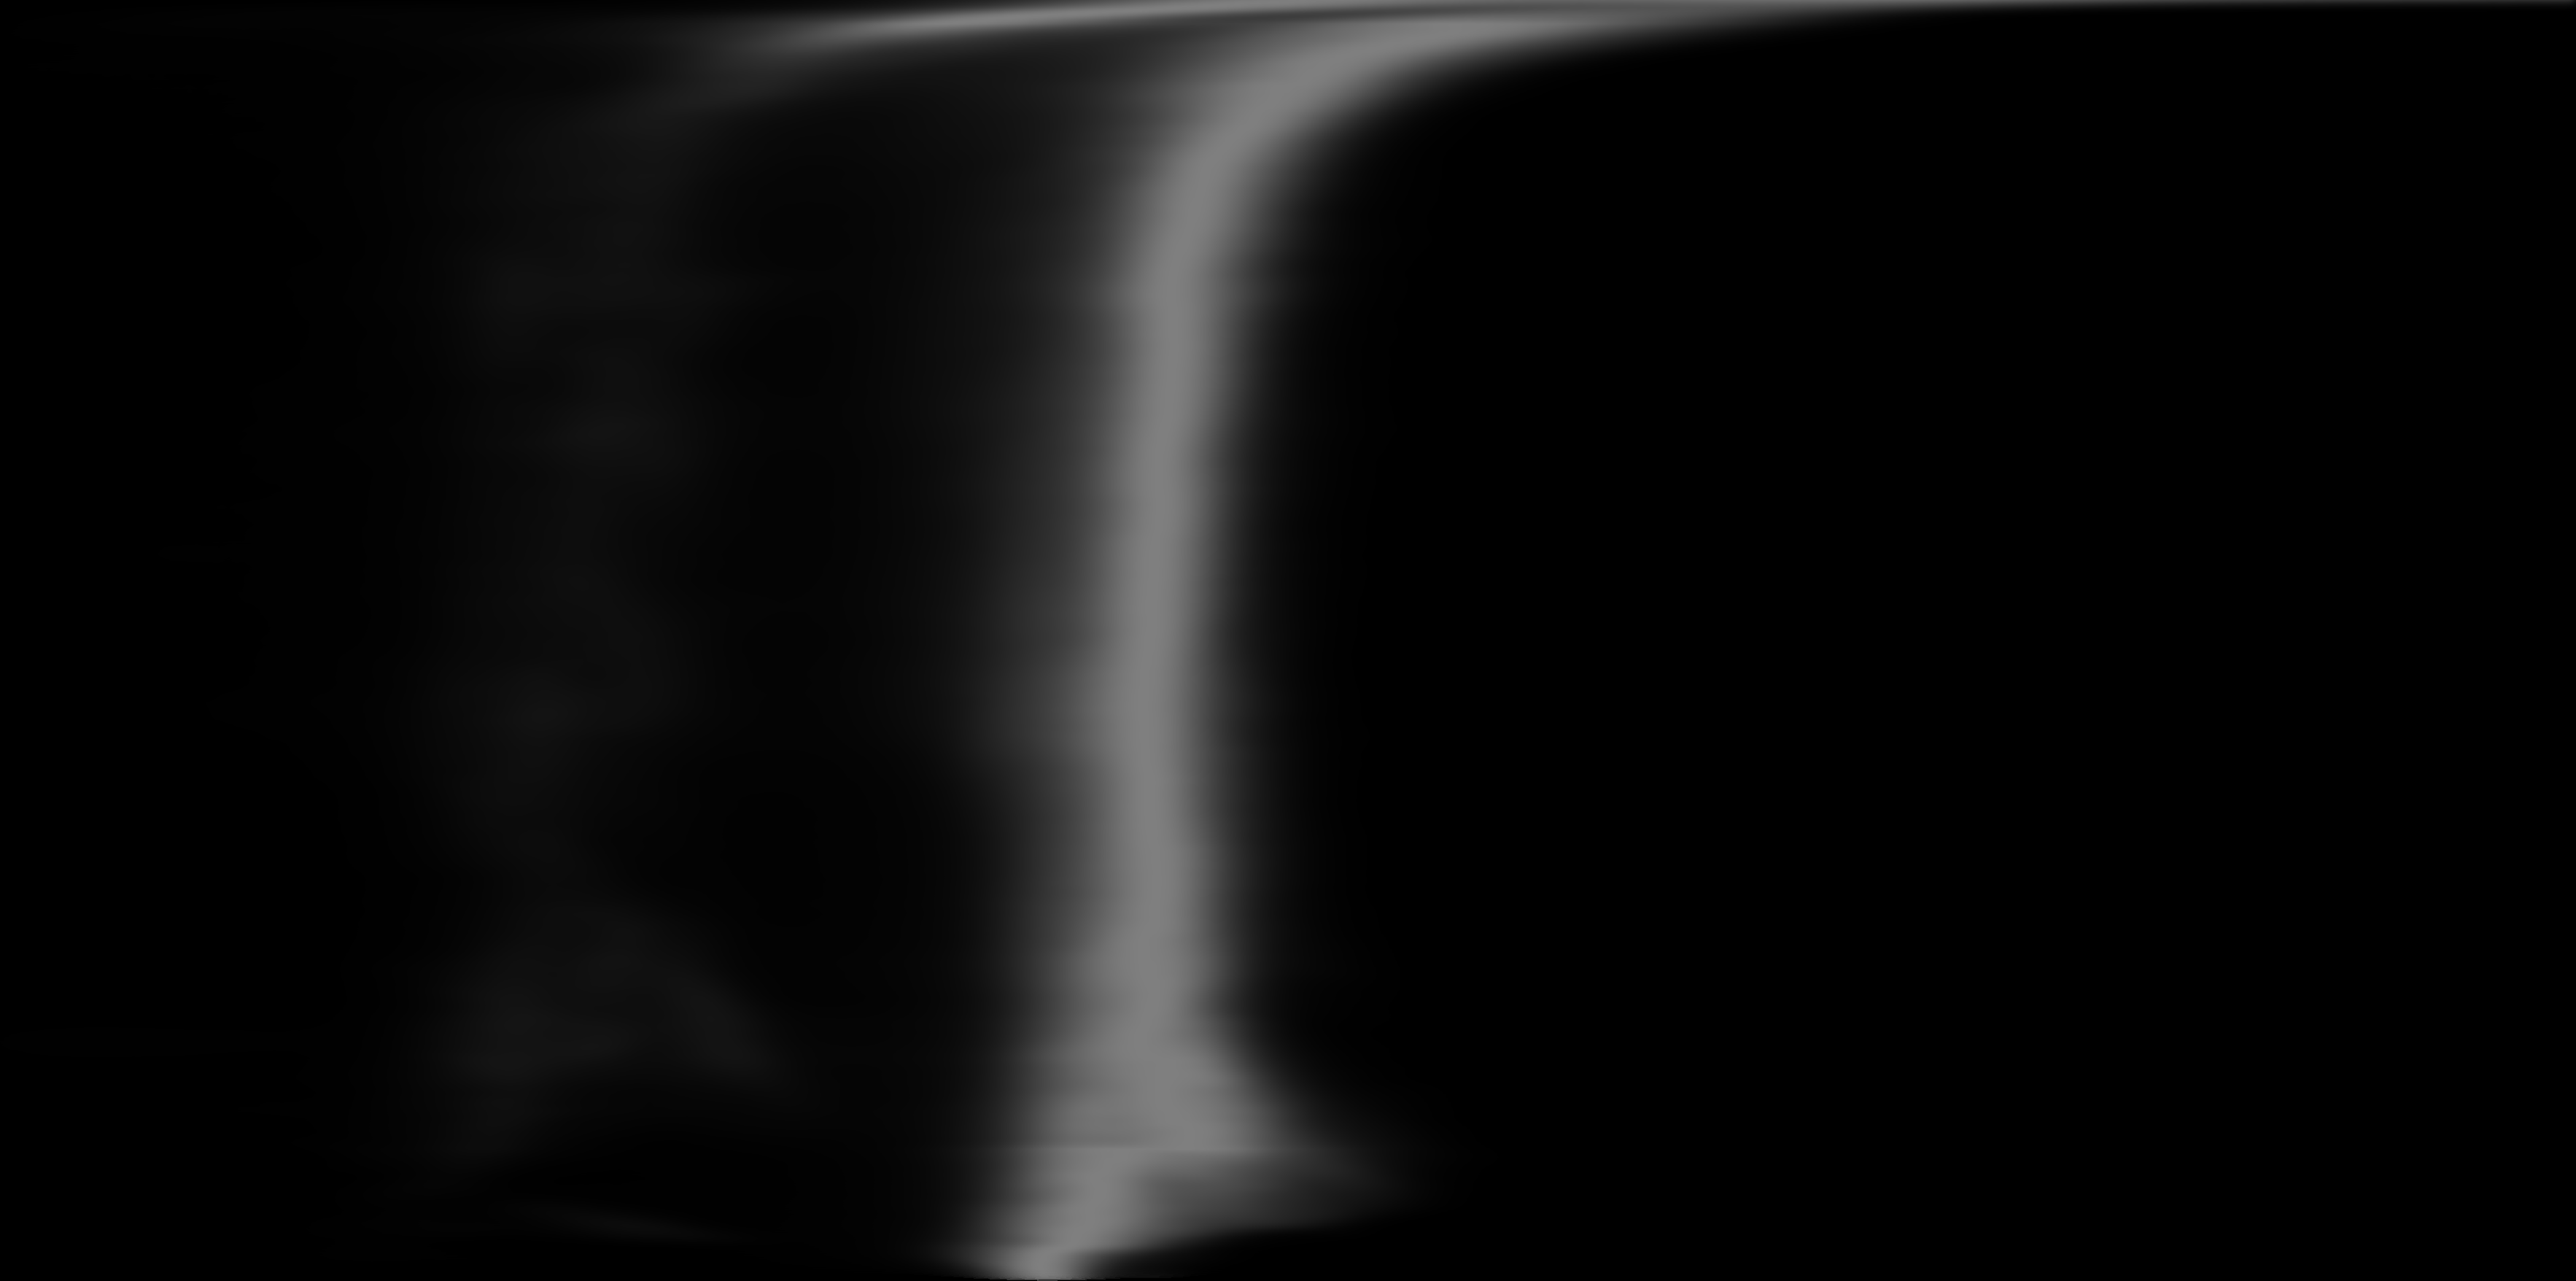
\includegraphics[width=\linewidth]{figures/fb-edt-bone_region3.png}
    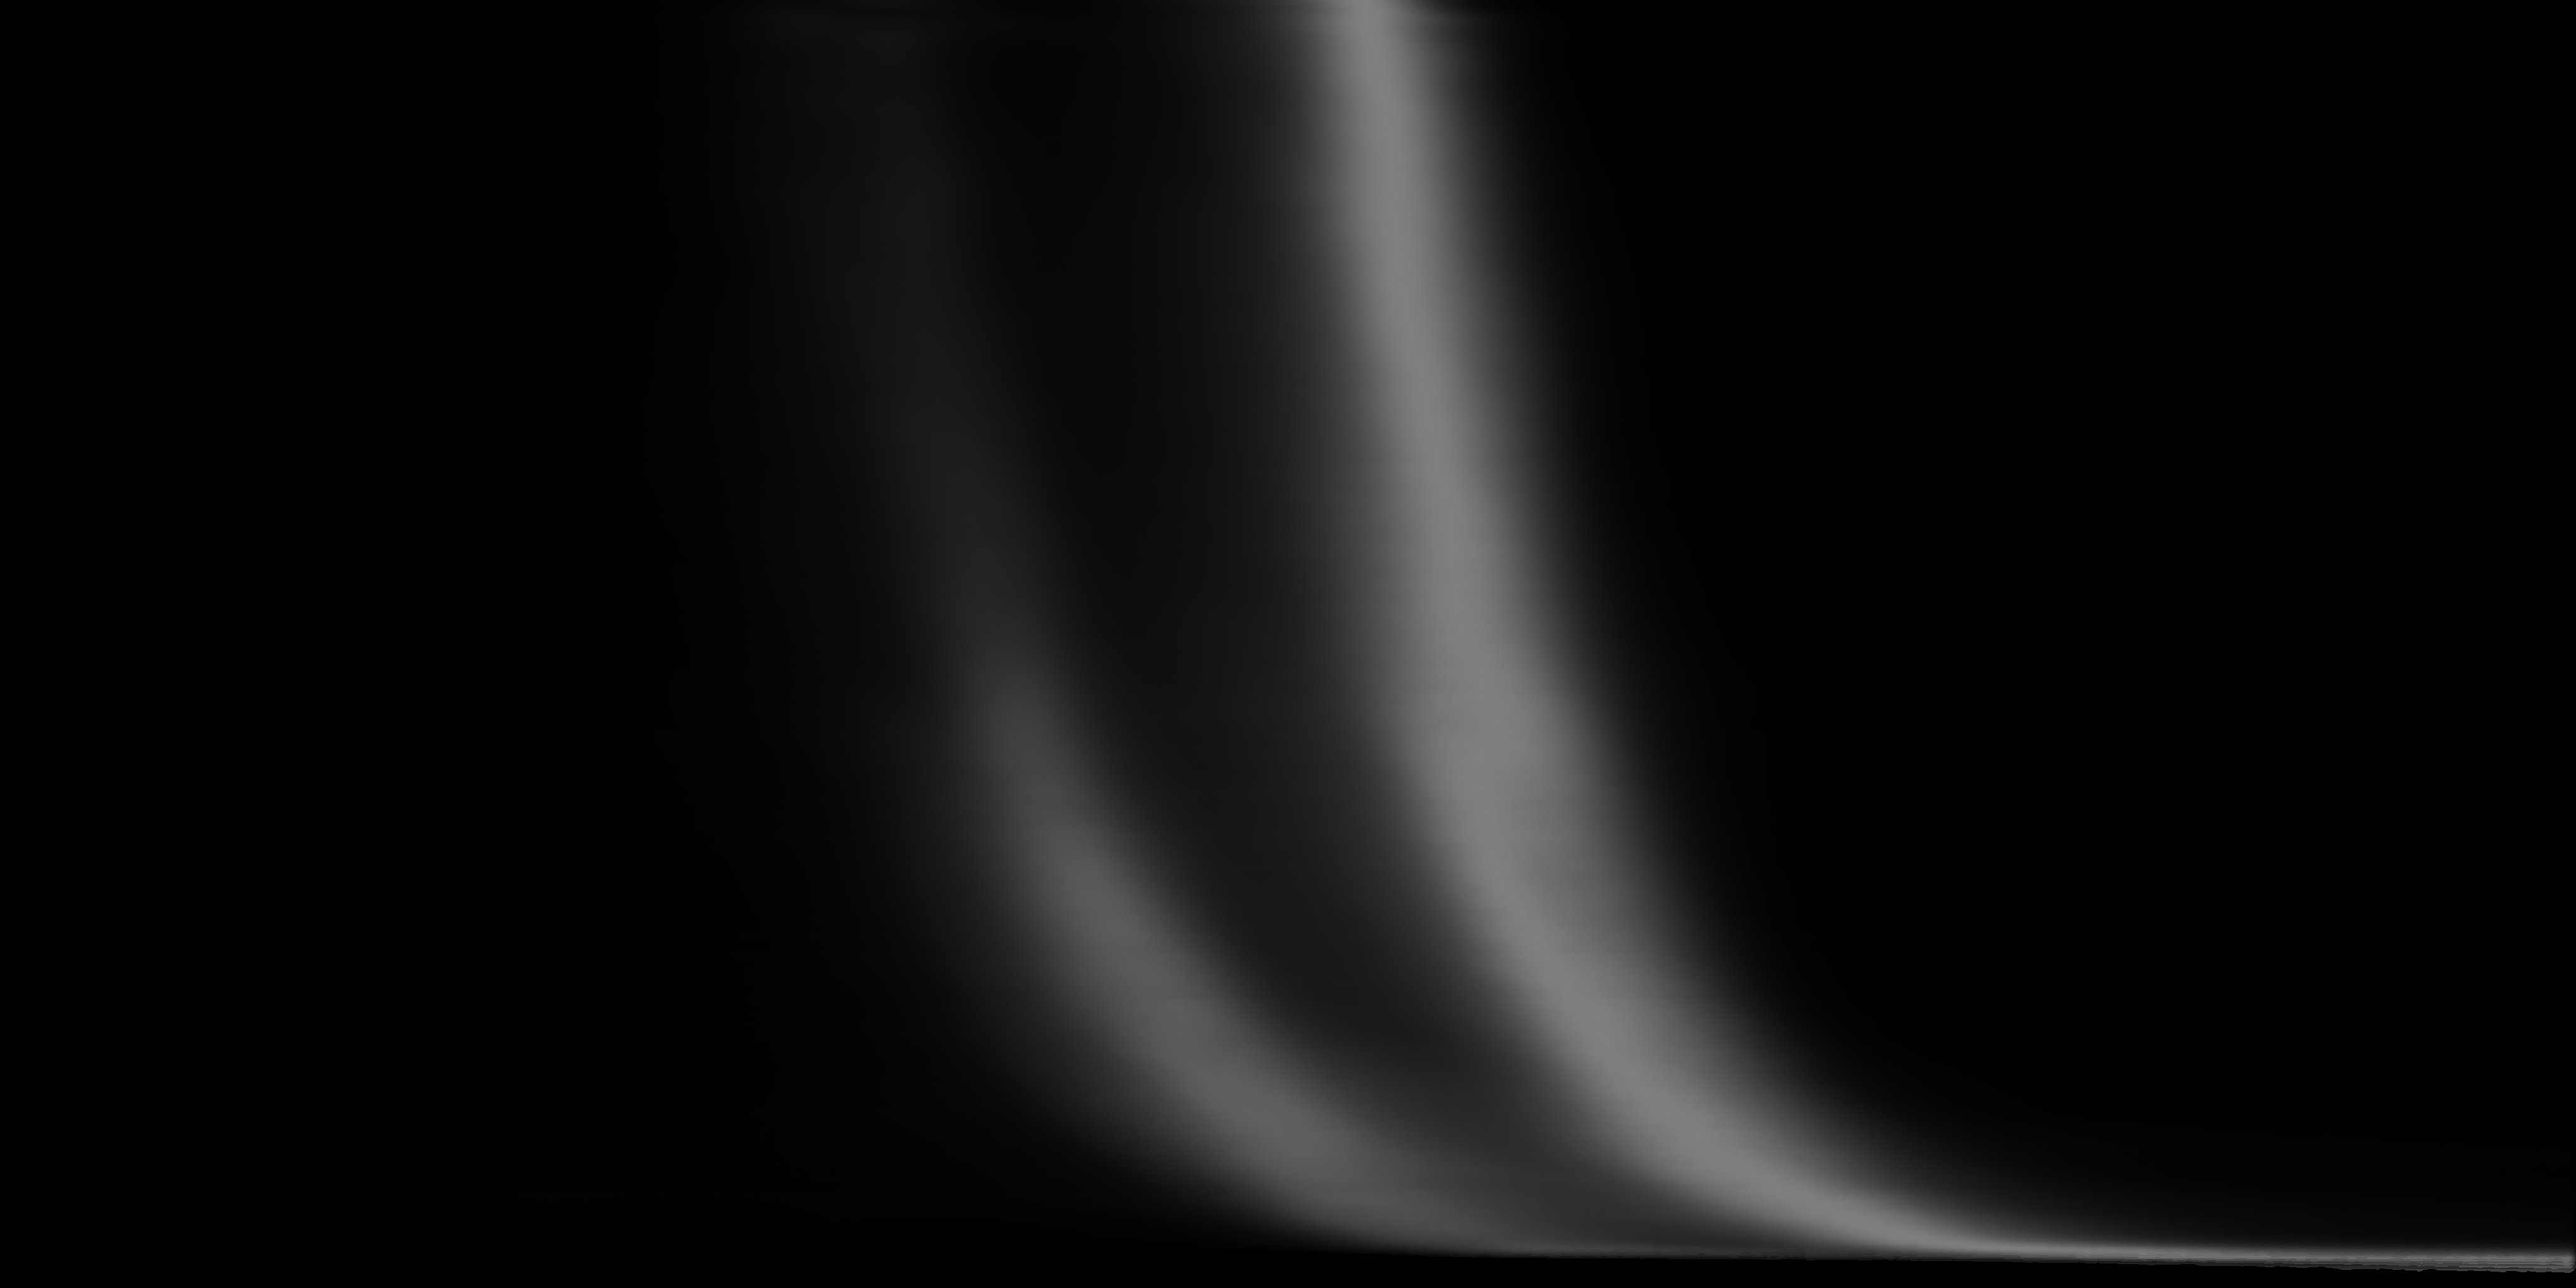
\includegraphics[width=\linewidth]{figures/fb-gauss-bone_region3.png}
    \carl{color scheme, axes.}
    \caption{2D field histogram. Note that there are two clearly seperated curves, which make up the different materials. Top is EDT, bottom is Diffusion.}
    \label{fig:field-hist}
\end{figure}

\vspace{\baselineskip}
\noindent\textbf{Isolate the materials} \\

The next step is to isolate the different materials spatially, which we do through the histogram.
As mentioned, we have two clearly defined curves making up the two materials.
To extract and label these curves, we apply the algorithm described in~\Cref{alg:material}.
Each contour becomes its own material, which is then labeled as material 1 and 2 respectively.

\begin{algorithm}
    \caption{Material isolation.}
    \label{alg:material}
    \begin{algorithmic}
        \Function {Materials} {$h[f_{bins},v_{bins},\sigma, peak_{min}, k_x, k_y, i_{dilate},$ \newline $i_{erode}, t]$}
            \State \textbf{allocate} $l[f_{bins},v_{bins}, ps[f_{bins},v_{bins}$]
            \For {$row$ \textbf{in} $0{:}f_{bins}$}
                \State $r \gets gaussian\_smooth(h[row,:], \sigma)$
                \State $p \gets find\_peaks(r, peak_{min})$
                \State $ps[p] \gets 1$
            \EndFor
            \State $kernel = cross\_kernel((k_x, k_y))$
            \State $d \gets dilate(ps, i_{dilate}, kernel)$
            \State $e \gets erode(d, i_{erode}, kernel)$
            \State $cs \gets find\_contours(e)$
            \For {$i$ \textbf{in} $0{:}|cs|$}
                \If {$size(cs[i]) > t$}
                    \State $l \gets draw\_contour(l, cs[i], i+1)$
                \EndIf
            \EndFor
            \Return $l$
        \EndFunction
    \end{algorithmic}
\end{algorithm}

\begin{figure}
    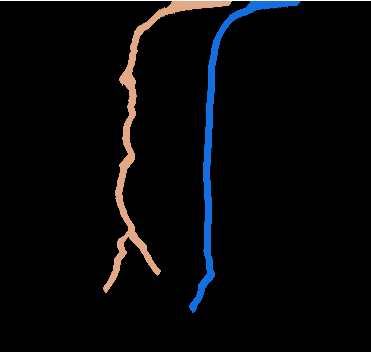
\includegraphics[width=\linewidth]{figures/curves_edt.png}
    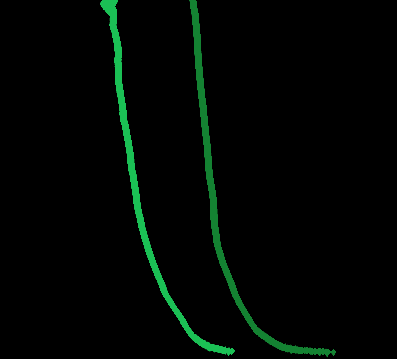
\includegraphics[width=\linewidth]{figures/curves_diffusion.png}
    \carl{intermediate images of all of the steps?}
    \caption{Curve finding intermediate steps. Top is EDT, bottom is Diffusion.}
    \label{fig:curves}
\end{figure}

\vspace{\baselineskip}
\noindent\textbf{Compute the probability distributions} \\

The curves are next use to restrict the model

\vspace{\baselineskip}
\noindent\textbf{Perform segmentation}

The final step of the segmentation process is to utilize the probabilities for segmentation.
This process is fairly straightforward, as each voxel is looked up in the probability distribution, which carries the same shape as the field histogram.

%\begin{figure}
%    \begin{lstlisting}[language=Python,caption=Python-like pseudo code for the final segmentation.,label=lis:segmentation]
%for z, y, x in indices:
%    v = voxel[z,y,x]
%    f = field[z,y,x]
%    result[z,y,x] = prob[f,v]
%    \end{lstlisting}
%\end{figure}

\begin{algorithm}
    \caption{Final segmentation from the probability distributions.}
    \label{alg:segment}
    \begin{algorithmic}
        \Function {Segment} {$voxels[n_z,n_y,n_x], p[f_{bins},v_{bins}],$ \newline $v_{bins}, v_{min}, v_{max}, f_{bins}, f_{min}, f_{max}$}
            \State \textbf{allocate} $result[n_z,n_y,n_x]$
            \For {$z,y,x$ \textbf{in} $0{:}n_z,0{:}n_y,0{:}n_x$}
                \State $v \gets voxels[z,y,x]$
                \If {$v_{min} \leq v \leq v_{max}$}
                    \State $f \gets voxels[z,y,x]$
                    \If {$f_{min} \leq f \leq f_{max}$}
                        \State $v_i \gets (v_{bins} - 1) - \frac{v - v_{min}}{v_{max} - v_{min}}$
                        \State $f_i \gets (f_{bins} - 1) - \frac{f - f_{min}}{f_{max} - f_{min}}$
                        \State $result[z,y,x] \gets p[f_i, v_i]$
                    \EndIf
                \EndIf
            \EndFor
            \Return $result$
        \EndFunction
    \end{algorithmic}
\end{algorithm}



\subsection{Results of the field segmentation}


\subsubsection{Visualizing bone-implant contact and blood-implant contact

}